\begin{frame}
\frametitle{Objectifs} 

L'objectif de ce groupe de travail est à partir de nombreux exercices, de créer des tactiques spécifiques à ce type d'exercice.

\end{frame}

\begin{frame}
\frametitle{Arbre de décision}
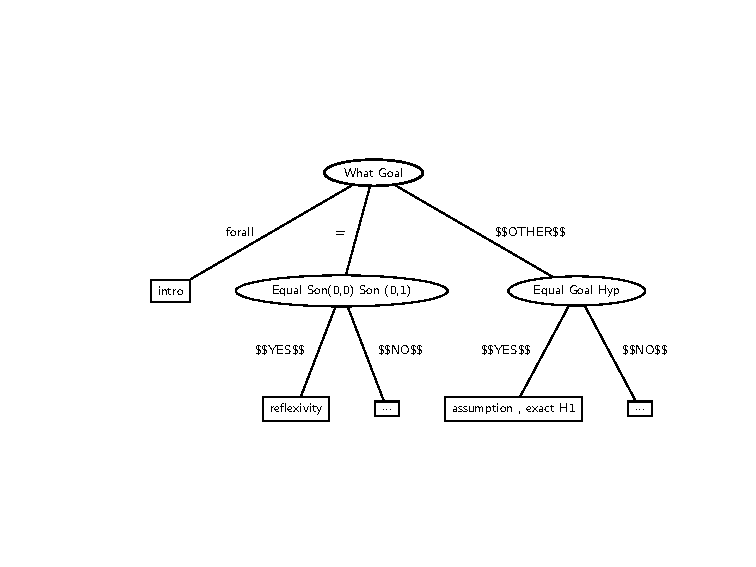
\includegraphics{../images/apprentissage/decision_tree.jpg}
\end{frame}

\begin{frame}
\frametitle{Découpage du workpackage}
\includegraphics[scale=0.2]{../images/apprentissage/organisation_apprentissage.pdf}
\end{frame}


\begin{frame}
  \frametitle{Acquisition}
  «en fonction du contexte (hypothèses+but), quelle tactique ?»
  \begin{itemize}
    \item analyse des fichiers {\tt .v}
      \begin{itemize}
        \item outils existants (XML) : inadaptés (contextes intermédiaires)
        \item lex+yacc : schéma général
        \item \textit{ad-hoc} : identificateurs dans chaque terme
      \end{itemize}
    \item analyse des fichiers {\tt .out} (sortie de coqtop) 
      \begin{itemize}
        \item \textit{ad-hoc} : schéma général très spécifique à coqtop
        \item lex+yacc : termes d'hypothèses et de but
      \end{itemize}
    \item combinaison contextes/tactiques
    \item traitement
      \begin{itemize}
        \item indices des variables dans le contexte (De Bruijn)
        \item forme spécifique à l'algorithme d'apprentissage
      \end{itemize}
  \end{itemize}
\end{frame}



\begin{frame}
\frametitle{L'apprentissage}
  \begin{definition}[entropie]
    L'entropie d'un tirage aléatoire est la longueur moyenne du code pour désigner la réponse : $\sum_{i \in I}{-p_i*\log{p_i}}$
  \end{definition}

  On cherche donc à diminuer l'entropie jusqu'à 0 grâce à des questions. 
 
  De plus, on veut avoir l'arbre le plus petit possible

  On choisit la question qui maximise la diminution d'entropie sur le nombre de réponse.

\end{frame}

\begin{frame}
  \frametitle{Difficultés}
  \begin{itemize}
  \item Grand nombre de questions possibles
  \item Multiplicité des réponses à une même question pour un même exemple
  \item Renumérotation des hypothèses
  \item Questions non fixes
  \end{itemize}
\end{frame}


\begin{frame}
  \frametitle{Pipeau?}
  \begin{itemize}
  \item Supposition d'une distribution représentative \\
    $\rightarrow$ Problèmes très classiques, redondant
  \item Pas l'arbre le plus petit en théorie \\
    $\rightarrow$ En pratique, ça marche
  \item Choix restreint sur les questions\\
    $\rightarrow$ Souvent comme ça qu'on réflechit
  \end{itemize}
\end{frame}


\begin{frame}
  \frametitle{Résultats}
  \begin{itemize}
  \item L'extraction de donnée est faite
  \item L'algorithme d'apprentissage est fait
  \item La décision à partir d'un problème et d'un arbre est faite
  \item Bonus 1 : Traduction en tactique
  \item Bonus 2 : On comprend ``apply H''
  \item Efficace?
\end{itemize}
\end{frame}

\begin{frame}
  \frametitle{Perspectives}
  
  \begin{itemize}
  \item Compréhension des termes : cut ( z + t = 10)
  \item Connexion avec l'IDE
  \item Bases d'exemples sur le net
  \item Update à la volée
  \item Pruning : quand les questions n'ont aucun sens
  \end{itemize}
\end{frame}
